
\documentclass[12pt]{article}

\usepackage{graphicx}
\usepackage{natbib}

\title{Enabling naturalistic, long-duration and continual animal experimentation}

\begin{document}

\maketitle

\section{Vision}

For over four years, at the Sainsbury Wellcome Centre and Gatsby Computational
Neuroscience Unit, we have been developing the AEON platform, a set of hardware
and software tools that support a new type of experimentation, where animals
are allowed to express ethologically-relevant behaviors, in naturalistic
environments, and in long-duration experiments, while their behavior and
neural activity is monitored continuously for weeks to months.
%
We have used this platform to characterize foraging behavior in both solitary
and groups of mice~\citep{aeonRepo} (Figure~\ref{fig:aeonPlatform}).

Our US partner, the Allen Institute for Neural Dynamics, is using the AEON
platform in continuous learning experiments, where mice freely explore odors
continuously for days to weeks~\citep{carlsPapers}.

This is an unprecedented type of experimentation that \ldots

Several groups around the world are performing this new type of
experimentation~\cite{}.

\begin{figure}
    \begin{center}
        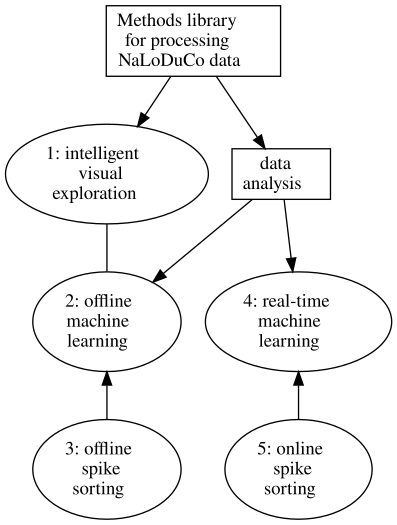
\includegraphics[width=5in]{figures/aims.png}
    \end{center}
    \caption{Proposal aims}
    \label{fig:aims}
\end{figure}

\subsection*{Aim 1: create software for visual exploration and statistical data
analysis of NaLoDuCo experimental data on the cloud}

Using the AEON platform we and others have recorded unprecedented data. We next
want to openly disseminate these data. However, this dissemination is not
trivial, as datasets generated by this new type of experimentation are
enormous. For instance, the size of a dataset generated from a one week
recording of behavioral and neural activity from a foraging mouse in SWC
experiments exceeds 200 terabytes. It will take users several days to download
these datasets over standard Internet connections.
%
So, instead of bringing data to users, we will bring users to data, by storing
datasets in the cloud, and providing \textbf{cloud software to allow users to visually
explore and statistically analyse behavioural and neural NaLoDuCo datasets
where they live} (Figure~\ref{fig:aims}, left box).

Our statistical analysis of neural time series will require knowledge of the
spiking activity of single units; i.e., spike sorting. In long-duration
experiments with freely moving animals spike sorting is a challenging problem,
because movements of recording probes change the shape of spike waveforms over
time and complicate the assignment of spikes to units based on spike waveforms.
We will address this problem by developing \textbf{spike sorting methods for
long-duration and continual, long-duration and high-channel-count recordings}
(Figure~\ref{fig:aims}, left box).

\subsection*{Aim 2: create real-time machine learning methods for intelligent
experimentation}

In small-animal Neuroscience, most often statistical processing of neural time series is
performed offline;
i.e., experimental data is collected, saved to files, which are later
statistically processed, with no runtime constraints. Most often all
experimental data is processes at the same time; i.e., batch processing.

A new online statistical processing approach is now emerging in small-animal Neuroscience,
where data is processes while it is being collected, and at the speed of data
generation~\citep{vermaniEtAl24}.

Online methods are well suited for NaLoDuCo experimentation. In experiments
extending for weeks to months animals learn and adapt, their motivation and
fatigue may fluctuate, and experimental conditions (e.g., lighting) may change.
Offline batch processing algorithms cannot model this type of changing data.
They assume stationary data whose statistical properties do not change across
time. Differently, most online processing algorithms are robust to
these changes.
%
Also, NaLoDuCo experimentation is well suited for online methods, as the
long-duration of these experiments provide a large amount of data to accurately
fit expressive online methods.

We will \textbf{optimize methods developed for Aim~1 so that they can operate
in real time}, and focus on the following two applications of these online
methods (Figure~\ref{fig:aims}, right box).

\subsubsection*{Intelligent neuromodulation}

Brain activity can be modulated optically, chemically and
electrically~\citep{}.
%
Most commonly this modulations is done at fixed experimental times, or based on
simple behavioral or neural observations.

We will guide optogenetic manipulations based on inferences from advanced
machine learning methods.
%
For example, a scientists may hypothesize that a peak in a neural latent
variable, inferred from a prefrontal cortex population, signals the moment when
mice decide to begin a foraging bout.  To test this, she runs an online machine
learning model to estimate latent variables from prefrontal cortex activity,
predicting when this peak will occur. She then optogenetically inactivates the
neural population at the forecasted time.  Because inactivation prevented the
mouse from initiating a foraging bout, her hypothesis is supported.

\subsubsection*{Intelligent experimental data storage}

As the duration of NaLoDuCo experiments become longer, and the richness of the                                                              
behavioral and neural recordings become larger, it will be unfeasible to                                                                
store all raw data. We will be forced to intelligently decide, in real time,                                                                
subsets of data to discard.
                                                                                                                                            
For instance, if we are recording videos from a mouse foraging in a large arena
with ten high-resolution cameras, it would save considerable storage if at any
time we only save videos from cameras capturing the mouse at that time.  This
could be done by tracking the position of the mouse in real time with
probabilistic machine learning methods. Then, when the confidence of the
tracking is high, we would only save videos of cameras capturing the mouse at
the tracked position, but when the confidence is low, we would save all videos.

\section{Approach}

\subsection{Offline data analysis on the cloud}

\end{document}
